\documentclass[11pt,a4paper,french,twoside]{PMCours}
\usepackage{hyperref}

\newcounter{activite}
\newcommand{\activite}{\subsubsection*{Activité~\refstepcounter{activite}\theactivite}}

\begin{document}
\TitreISN{Classe de Terminale}{Année 2021--2022}
{Numérique et Sciences Informatiques}{Entrainement à l'\'Epreuve de Spécialité - Sujet 2 - 3h30}
\ \medskip\\
{\large Chaque candidat traitera trois exercices au choix parmi les quatre proposés, chaque exercice étant noté sur sept points.\medskip\\
L'usage de tout document, calculatrice, etc... est interdit. \medskip\\
Les élèves rendront de manière impérative brouillons et sujet en même temps que leur composition.}

%\tableofcontents

%
%
%
%
\newpage\noindent
\section*{Exercice 1}
\emph{Cet exercice porte sur le maniement de listes Python et sur des questions liées à l'algorithmique.}\medskip\\
Dans tout cet exercice, les éléments des tableaux sont tous de type numérique \code{int} ou \code{float}.
\begin{enumerate}
\item On se donne la fonction suivante, prenant comme paramètre un tableau Python \code{t}.
\begin{Python}
def test(t) :
	n = len(t)
	for k in range(n-1) : 
		if t[k] > t[k+1] :
			return False
	return True
\end{Python}
\begin{enumerate}
\item Que renvoie les appels \code{test([1,3,2])} et \code{test([1,2,3])} ?
\item Dans quel cas exécute-t-on la ligne \code{6} ? 
\item Quel est le but de cette fonction ? 
\item Justifier l'utilisation de \code{range(n-1)} au lieu de \code{range(n)} en ligne \code{3}.
\end{enumerate}
\item On se donne l'algorithme suivant dans lequel \code{a} et \code{b} sont deux tableaux triés dans l'ordre croissant et dont les éléments sont indexés de manière classique, c'est à dire à partir de $0$.\\
Son but ultime est de renvoyer un tableau trié contenant tous les éléments de \code{a} et de \code{b}. 
\begin{Python}
Fonction fusion(a,b)
m=longueur(a)
n=longueur(b)
t=[]
i=0
j=0
Tant que i<m et j<n
	Si a[i]<b[j]
	Alors 
		t reçoit a[i]
		i=i+1  
	Sinon 
		t reçoit b[j]    
		j=j+1
Renvoyer(t)
\end{Python}
\begin{enumerate}
\item Implémenter la fonction \code{fusion} en langage Python.
\item Remplir le tableau suivant (on pourra recopier les cases concernées du tableau ou joindre la feuille) décrivant le déroulement de l'exécution de \code{fusion(a,b)} avec \code{a=[-1,4,5]} et \code{b=[2,3,7,8]}.\medskip\\
.\hskip-3cm{\large \begin{tabular} {|l|p{2.1cm}|p{1.9cm}|p{1.9cm}|p{1.9cm}|p{1.9cm}|p{1.9cm}|p{1.9cm}|}\hline
\code{init.}&\multicolumn{7}{l|}{\code{m=3} \hskip5mm \code{n=4}\hskip5mmt=[ ]\hskip5mm \code{i=0}\hskip5mm \code{j=0}}\\ \hline
{\small\code{boucle T.que}}&&{\small1$^{er}$ passage}&{\small$2^{em}$ passage}& &&& \\ \hline
\code{test T.que}&i<m et j<n&{\small 0<3\&0<4}\code{:V}&{\small 1<3\&0<4}\code{:V}& &&& \\ \hline
\code{test Si} &a[i]<b[j]&{\small -1<2}\code{:V}&{\small 4<2}\code{:F}&&& & \\ \hline
                               &t             &t=[-1] &t=[-1,2]&& && \\ \hline
                               &i             &i=1 &i=1 && && \\ \hline
                               &j             &j=0 &j=1&&& & \\ \hline
{\small\code{fin T.que}}&\multicolumn{7}{l|}{}\\ \hline
 \end{tabular}}
\item Si on laisse le programme en l'état, justifier brièvement que \code{t} ne contient pas tous les éléments de \code{a} et de \code{b}.
\item Ajouter les instructions nécessaires (ne recopier que les nouvelles lignes mais indiquer le niveau d'indentation) pour que après exécution de \code{fusion(a,b)}, le tableau \code{t} contienne tous les éléments de \code{a} et de \code{b}.\medskip\\
On signale que si \code{t} est un tableau Python et \code{i} un type \code{int} de valeur $\geq 0$, alors \code{t[i:]} contient tous les éléments de \code{t} d'indice supérieur ou égal à \code{i} et est vide si \code{i}$\geq$ \code{len(t)}.
\item Donner alors directement sans justification \code{fusion(a,b)} lorsque \code{a=[-3,2,4,7,9]} et \code{b=[-1,2,3,5]}.
\end{enumerate}
\item 
\begin{enumerate}
\item Ecrire une fonction Python \code{transf} prenant comme paramètre un tableau Python \code{t} et renvoyant un tableau de même longueur mais dont les éléments sont des tableaux de longueur 1.\\
Ainsi, \code{transf([2,-1,4])} renvoie \code{[ [2] , [-1] , [4] ]}.
\item Ecrire une fonction Python \code{detransf} prenant comme paramètre un tableau Python  \code{tt} dont les éléments sont des tableaux et renvoyant un unique tableau contenant les mêmes éléments.\\
Ainsi, \code{detransf( [ [2,3] , [-1] , [-1,3,4] ] )} renvoie \code{[2,3,-1,-1,3,4]}.\\
On rappelle que en Python, l'instruction \code{[2,3]+[-1]} construit le tableau \code{[2,3,-1]}
\item On se donne alors le code suivant : 
\begin{Python}
def mystere(t) :
	tt = transf(t)
	T = tt[0]
	for i in range(1,len(tt)) :
		T=fusion(T,tt[i])
	return T
\end{Python}
Expliquer en justifiant brièvement ce que fait la fonction \code{mystere} si on l'applique à un tableau \code{t}.
\end{enumerate}
\end{enumerate}
\newpage\noindent
\section*{Exercice 2}
\emph{Cet exercice porte sur les bases de données relationnelles et le langage SQL} \medskip\\

L'énoncé de cet exercice utilise les mots du langage SQL suivant :
\begin{verbatim}
SELECT, FROM, WHERE, JOIN, INSERT INTO, VALUES, ORDER BY, DISTINCT, COUNT
\end{verbatim}

On s'intéresse à l'organisation d'un lycée. Un responsable de lycée doit concevoir une base de données afin de gérer au mieux l'occupation des salles de cours, et s'assurer de la disponibilité des salles informatiques en particulier. Pour cela, il a conçu une base de données relationnelle avec quatre relations, dont des extraits sont fournis ci-après (où le symbole \verb'#' désigne une clé étrangère) :

\begin{itemize}
\item \verb'Classe' (\underline{nom} : String, \verb'prof_princ' : String, \verb'niveau' : String)

\item \verb'Eleve' (\underline{id} : Int, \verb'nom' : String, \verb'#classe' : String, \verb'LV1' : String, \verb'spé1' : String, \verb'spé2' : String)

\item \verb'Salle' (\underline{num} : Int, \verb'nb_de_places' : Int, \verb'salle_info' : Boolean)

\item \verb'Cours_de_spé' 
\end{itemize}

\begin{figure}[h]
\begin{center}
\begin{tabular}[c]{|c|c|c|}\hline
\verb'nom' & \verb'prof_princ' & \verb'niveau'  \\\hline
TG1 & M. Durand & terminale  \\\hline
1G3 & Mme Hubert & première   \\\hline
TG4 & Mme Chipo & terminale   \\\hline
\end{tabular}
\end{center}
\caption{Extrait de la relation \textbf{Classe}}
\end{figure}

\begin{figure}[h]
\begin{center}
\begin{tabular}[c]{|c|c|c|c|c|c|}\hline
\verb'id' & \verb'nom' & \verb'classe' & \verb'LV1' & \verb'spé1' & \verb'spé2'\\\hline
144 & Bilout & TG4 & anglais & maths & nsi\\\hline
213 & Zidane & TG4 & allemand & maths & physique\\\hline
145 & Dugenou & 1G1 & anglais & physique & nsi\\\hline
56 & Dubras & TG2 & anglais & physique & svt\\\hline
\end{tabular}
\end{center}
\caption{Extrait de la relation \textbf{Eleve}}
\end{figure}

\begin{figure}[h]
\begin{center}
\begin{tabular}[c]{|c|c|c|}\hline
\verb'num' & \verb'nb_de_places' & \verb'salle_info'  \\\hline
B51 & 24 & true  \\\hline
C38 & 24 & false   \\\hline
B13 & 12 & true   \\\hline
\end{tabular}
\end{center}
\caption{Extrait de la relation \textbf{Salle}}
\end{figure}

\begin{figure}[h]
\begin{center}
\begin{tabular}[c]{|c|c|c|c|}\hline
\verb'matière' & \verb'jour' & \verb'horaire' & \verb'salle'  \\\hline
nsi & mardi & 10:00 & B51  \\\hline
nsi & mardi & 10:00 & B13  \\\hline
maths & mercredi & 10:00 & C38  \\\hline
physique & lundi & 14:00 & C38  \\\hline
\end{tabular}
\end{center}
\caption{Extrait de la relation \textbf{Cours\_de\_spé}}
\end{figure}



On suppose, pour simplifier, que tout élève de lycée a choisi deux spécialités réparties arbitrairement entre \verb'spé1' et \verb'spé2'.

\begin{enumerate}

\item D'après vous, à quel concept des bases de données relationnelles le soulignement du nom d'un attribut fait-il référence ?


\item Pour la relation \verb'Cours_de_spé', au vu des enregistrements présentés, comment définiriez-vous ce concept ? Vous écrirez votre proposition à l'aide de noms d'attributs, séparés par une virgule, groupés avec des parenthèses. L'ordre n'importe pas. Justifiez votre réponse.

\item Comment qualifie-t-on l'attribut \verb'salle' de la relation \verb'Cours_de_spé', sachant qu'un numéro de salle doit forcément faire référence à une salle de cours de la relation \verb'Salle' ?

\item Ecrire le schéma relationnel de la relation \verb'Cours_de_spé'. On rappelle que les types SQL sont : Int, Float, String, Time, Boolean.

\item Quel résultat renvoie l'exécution de la requête SQL suivante, sur l'extrait de la relation \verb'Eleve' donné ci-dessus ? 
\begin{verbatim}
SELECT nom, classe FROM Eleve WHERE LV1 = "anglais"
\end{verbatim}


\item Ecrire une requête SQL qui affiche l'id et le nom des élèves qui ont choisi la spécialité \verb'nsi'.


\item Une nouvelle classe de première va ouvrir l'année prochaine. Son nom sera \verb'1G8' avec comme professeur principal \verb'M. Strong'. Ecrire une requête pour ajouter ces informations dans la relation \verb'Classe'.

\item Ecrire une requête SQL qui affiche la matière dont le cours de spécialité est le plus matinal du jeudi dans la salle C14. On pourra utiliser notamment la commande SQL \verb'LIMIT 1' qui renvoie la première ligne d'un résultat d'une requête SQL.


\item Ecrire une requête SQL qui affiche le nom de tous les élèves de terminale qui font LV1 allemand, avec le nom de leur professeur principal associé.


\item Ecrire une requête SQL qui renvoie le nombre de salles informatiques occupées chaque jeudi à 11h00.


\item Que renvoie la requête SQL suivante ? Formulez votre réponse le plus simplement possible (cela tient sur une ligne !).
\begin{verbatim}
SELECT nom FROM Eleve
WHERE spé1 IN (
SELECT matière FROM Cours_de_spé
JOIN Salle ON Salle.num = Cours_de_spé.salle
WHERE Salle.salle_info = true
AND Cours_de_spé.jour = "jeudi"
) OR spé2 IN (
SELECT matière FROM Cours_de_spé
JOIN Salle ON Salle.num = Cours_de_spé.salle
WHERE Salle.salle_info = true
AND Cours_de_spé.jour = "jeudi"
)
\end{verbatim}


\end{enumerate}

\newpage\noindent
\section*{Exercice 3}
\emph{Cet exercice traite principalement le thème \og{} algorithmique
langages et programmation\fg{}.} \medskip\\

L'objectif de cet exercice est de définir un moyen de de définir l'ordre 
d'exécution des processus dans un système d'exploitation multitâche sur un 
ordinateur ayant un unique processeur. En effet, le système doit assurer
l'exécution d'un nombre important de tâches, mais cele-ci ne peuvent être
assignées au processeur qu'une par une. De plus, les tâches ont des priorités
différentes. Dans un système d'exploitation, c'est le trvail de l'ordonnanceur.

\medskip
On choisit de représenter la file d'attente des processus à exécuter par 
un tableau (type \code{list}) dont les éléments sont de objets définis 
par la classe suivante :
\begin{Python}
class Processus:
    def __init__(self, nom, chemin, duree, priorite):
        self.nom=nom
        self.chemin=chemin
        self.duree=duree
        self.priorite=priorite
\end{Python}
Chaque processus est donc défini par son nom, son chemin, sa durée (en cycles 
d'horloge) et le niveau priorité (qui est un entier de $1$ à $10$, 
$1$ correspondant à une très faible priorité et $10$ à une tâche ultra prioritaire,
autrement dit : une tâche temps réel). 

\begin{enumerate}
    \item On exécute une à une les instructions suivantes :
\begin{Python}
attente=[]
attente.append(Processus("zip.exe","C:/bin",100,1))
attente.append(Processus("chrome.exe","C:/bin",50,6))
attente.append(Processus("skype.exe","C:/users/eve",60,9))
\end{Python}
\begin{enumerate}
    \item Quel est le résultat de l'exécution de \code{L[2].duree} ?
    \item Quel est le résultat de l'exécution de \code{L[1].chemin[2]} ?
    \item Quelle commande exécuter pour passer la priorité de skype à $10$ ?
\end{enumerate}    
    \item On considère la fonction suivante:
\begin{Python}
def mystere(attente):
    D=0
    for k in range(len(attente)):
        if attente[k].duree<D:
            D=attente[k].duree
    return D
\end{Python}
    Pour une liste \code{attente} d'objets de classe \code{Processus} quelconque,
    que fait cette fonction ?
    \item Écrire (en s'inspirant de la question précédente) une fonction 
    \code{tache\_critique(attente)} qui détermine
    le processus le plus prioritaire ou, s'il y a égalité, celui qui dure le 
    plus longtemps.
    Cette fonction doit retourner le rang du processus en question dans 
    la liste \code{attente}.
    \item On exécute une à une les instructions suivantes :
\begin{Python}
attente=[]
attente.append(Processus("zip.exe","C:/bin",100,1))
attente.append(Processus("chrome.exe","C:/bin",50,6))
attente[0]=attente[1]
attente[1]=attente[0]
\end{Python}
    Choisissez une réponse parmi les cinq suivantes :
    \begin{enumerate}
        \item La liste \code{attente} contient deux fois le processus zip.exe. 
        \item La liste \code{attente} contient deux fois le processus chrome.exe. 
        \item La liste \code{attente} est inchangée. 
        \item Les processus zip.exe et chrome.exe ont échangé leur place dans 
        la liste \code{attente}. 
        \item Une erreur se produit à l'exécution. 
    \end{enumerate}
    \item On exécute une à une les instructions suivantes :
\begin{Python}
attente=[]
attente.append(Processus("zip.exe","C:/bin",100,1))
attente.append(Processus("chrome.exe","C:/bin",50,6))
x=attente[1]
attente[1]=attente[0]
attente[0]=x
\end{Python}
    Choisissez une réponse parmi les cinq suivantes :
    \begin{enumerate}
        \item La liste \code{attente} contient deux fois le processus zip.exe. 
        \item La liste \code{attente} contient deux fois le processus chrome.exe. 
        \item La liste \code{attente} est inchangée. 
        \item Les processus zip.exe et chrome.exe ont échangé leur place dans 
        la liste \code{attente}. 
        \item Une erreur se produit à l'exécution. 
    \end{enumerate}
    \item Écrire une fonction \code{depasser(attente,k)}, qui compare les processus
    correspondants aux index $k-1$ et $k$ et les échange éventuellement pour que
    le prcessus le plus prioritaire (le plus court, s'ils ont la même priorité) 
    soit en position $k-1$.
    \item Écrire une fonction \code{suivant(attente)}, qui appliqué la fontion 
    \code{depasser} à toute la file d'attente, en commençant par les plus petits 
    index. Puis renvoie le premier processus en le retirant la liste.
    \item On souhaite modifier la fonction \code{depasser(attente,k)} pour qu'elle
    déplace le processus d'index $k$ vers la gauche et ce tant que le total des 
    priorités des processus qu'il dépasse est strictement inférieur 
    à son propre niveau de priorité. (Un processus de priorité $8$ pourra 
    dépasser les trois processus qui le précèdent si leurs priorités sont $1$, $4$, $2$, 
    mais il s'arrêtera là car $1+4+2=7<8$.)
    
    Compléter le code suivant :
\begin{Python}
def depasser(attente,k):
    p=attente[k].priorite
    i=k-1
    S=0
    while ____ and ________________:
        S=S+attente[i].priorite
        attente[i],attente[i+1]=_________________________
        i=___
\end{Python}
\end{enumerate}

\newpage\noindent

\section*{Exercice 4}
\emph{Cet exercice porte sur }\\





\end{document}





\newpage
\section*{Exercice 1}
\emph{Cet exercice porte sur les piles et leur implémentation en langage Python.}\\

\includegraphics[width=18cm]{images/page1.png}

\ \\

\includegraphics[width=17.5cm]{images/page2.png}

\includegraphics[width=18cm]{images/page3.png}
\includegraphics[width=17cm]{images/page4.png}



%
%
%
%
\newpage
\section*{Exercice 2}
\emph{Cet exercice porte sur les graphes et leur implémentation en langage Python.}\\
On rappelle que les graphes peuvent être représentés par des matrices d'adjacences ou par des dictionnaires. \medskip\\
\begin{tabular}{p{5cm}p{4cm}p{9.3cm}}
Par exemple, le graphe &correspond à la matrice&et au dictionnaire \\\\\
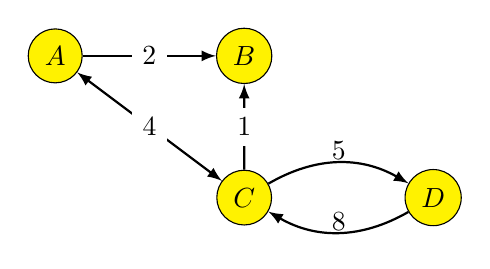
\begin{tikzpicture}[xscale=.6,yscale=.6]
% Styles (MODIFIABLES)
\tikzstyle{fleche}=[<->,>=latex,thick]
\tikzstyle{sfleche}=[->,>=latex,thick]
\tikzstyle{noeud}=[fill=yellow,circle,draw]
\tikzstyle{feuille}=[fill=orange,circle,draw]
\tikzstyle{etiquette}=[midway,fill=white,draw=white]
\tikzstyle{etiquette2}=[rectangle,fill=white,draw=white]
% Dimensions (MODIFIABLES)
\def\DistanceInterNiveaux{3}
\def\DistanceInterFeuilles{2}
% Dimensions calculées (NON MODIFIABLES)
\def\NiveauA{(-0)*\DistanceInterNiveaux}
\def\NiveauB{(-1)*\DistanceInterNiveaux}
\def\InterFeuilles{(1)*\DistanceInterFeuilles}
% Noeuds (MODIFIABLES : Styles et Coefficients d'InterFeuilles)
\node[noeud] (A) at ({(0)*\InterFeuilles},{\NiveauA}) {$A$};
\node[noeud] (B) at ({(2)*\InterFeuilles},{\NiveauA}) {$B$};
\node[noeud] (C) at ({(2)*\InterFeuilles},{\NiveauB}) {$C$};
\node[noeud] (D) at ({(4)*\InterFeuilles},{\NiveauB}) {$D$};
\node[etiquette2] (e1) at (6,-2) {5};
\node[etiquette2] (e1) at (6,-3.5) {8};
% Arcs (MODIFIABLES : Styles)
\draw[sfleche] (A)--(B) node[etiquette] {$2$} ;
\draw[fleche] (A)--(C) node[etiquette] {$4$} ;
\draw[sfleche] (C)--(B) node[etiquette] {$1$};
\draw[sfleche] (C) to [bend left] (D);
\draw[sfleche] (D) to [bend left] (C);
\end{tikzpicture}
&.\vskip -3cm$T=\left(\begin{array}{cccc}
0&2&4&0\medskip\\
0&0&0&0\medskip\\
4&1&0&5\medskip\\
0&0&8&0\medskip\\
\end{array}\right)  $
&
.\vskip -3cm \begin{Python}
di={'A':{'B':2,'C':4}, 
'B':{}, 
'C':{'A':4,'B':1,'D':5}, 
'D':{'C',8}}
\end{Python}

\end{tabular}
\subsection*{Question 1}
\begin{enumerate}
\item Donner la matrice d'adjacence et le dictionnaire correspondant au graphe : \medskip\\
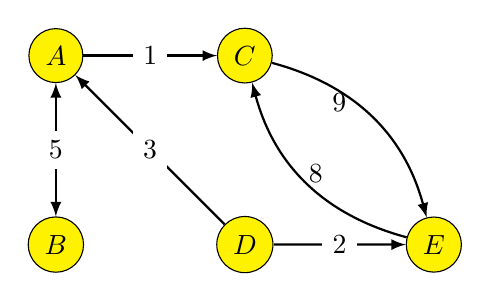
\begin{tikzpicture}[xscale=.6,yscale=.6]
% Styles (MODIFIABLES)
\tikzstyle{fleche}=[<->,>=latex,thick]
\tikzstyle{sfleche}=[->,>=latex,thick]
\tikzstyle{noeud}=[fill=yellow,circle,draw]
\tikzstyle{feuille}=[fill=orange,circle,draw]
\tikzstyle{etiquette}=[midway,fill=white,draw=white]
\tikzstyle{etiquette2}=[rectangle,fill=white,draw=white]
% Dimensions (MODIFIABLES)
\def\DistanceInterNiveaux{4}
\def\DistanceInterFeuilles{2}
% Dimensions calculées (NON MODIFIABLES)
\def\NiveauA{(-0)*\DistanceInterNiveaux}
\def\NiveauB{(-1)*\DistanceInterNiveaux}
\def\InterFeuilles{(1)*\DistanceInterFeuilles}
% Noeuds (MODIFIABLES : Styles et Coefficients d'InterFeuilles)
\node[noeud] (A) at ({(0)*\InterFeuilles},{\NiveauA}) {$A$};
\node[noeud] (C) at ({(2)*\InterFeuilles},{\NiveauA}) {$C$};
\node[noeud] (B) at ({(0)*\InterFeuilles},{\NiveauB}) {$B$};
\node[noeud] (D) at ({(2)*\InterFeuilles},{\NiveauB}) {$D$};
\node[noeud] (E) at ({(4)*\InterFeuilles},{\NiveauB}) {$E$};
\node[etiquette2] (e1) at (6,-1) {9};
\node[etiquette2] (e1) at (5.5,-2.5) {8};
% Arcs (MODIFIABLES : Styles)
\draw[fleche] (A)--(B) node[etiquette] {$5$} ;
\draw[sfleche] (A)--(C) node[etiquette] {$1$} ;
\draw[sfleche] (D)--(A) node[etiquette] {$3$};
\draw[sfleche] (D)--(E) node[etiquette] {$2$};
\draw[sfleche] (C) to [bend left] (E);
\draw[sfleche] (E) to [bend left] (C);
\end{tikzpicture}
\item \ \\
.\vskip -1cm \begin{tabular}{p{10cm}p{5cm}} Représenter le graphe dont les sommets sont nommés \code{'V','W','X','Y','Z'} et correspondant à la matrice d'adjacence &
$T=\left(\begin{array}{ccccc}
0&1&0&0&3\medskip\\
4&0&0&0&0\medskip\\
1&2&0&3&4\medskip\\
0&1&5&0&0\medskip\\
3&0&0&0&0\medskip\\
\end{array}\right) $
\end{tabular}
\item On considère un graphe représenté par un dictionnaire \code{di}.
\begin{enumerate}
\item Uniquement pour cette question, on prend pour \code{di} le dictionnaire de l'exemple introductif. Que renvoient les commandes suivantes ? \\
\code{len(di)} \hskip 1 cm  \code{di['D']} \hskip 1 cm  \code{len(di['C'])} \hskip 1 cm  \code{di['C']['B']} \hskip 1 cm  \code{di['A']['D']}\medskip \\
\hskip -6mm On revient maintenant au cas général.
\item Donner une commande simple permettant d'obtenir le nombre de sommets du graphe.
\item Si \code{s} est un sommet du graphe, donner une commande simple permettant d'obtenir le nombre d'arcs au départ de \code{s}.
\item Décrire ce que fait la fonction \code{f} suivante : 
\begin{Python}
def f(di):
	S=0
	for sommet in di :
		S=S+len(di[sommet])
	return S
\end{Python}
\item En adaptant la fonction \code{f}, construire une fonction \code{longueur\_graphe} prenant comme argument un dictionnaire d'adjacence \code{di} et renvoyant la somme de toutes les longueurs/poids des arcs du graphe (en sachant que comme ici les graphes sont non orientés, si \code{'A'} et \code{'B'} sont reliés dans les deux sens par une liaison de poids 5,  on comptera donc 5+5=10 dans la somme). 
\end{enumerate}
\end{enumerate}
.\vskip - 7 mm On donne maintenant une implémentation de la structure de graphe non orienté. Pour un tel graphe \code{G}, si \code{s} est un sommet de \code{G}, on appelle 
\begin{itemize}
\item successeur de \code{s} tout sommet de \code{G} que l'on peut atteindre à partir de \code{s}.
\item prédécesseur de \code{s} tout sommet de \code{G} à partir duquel on peut atteindre \code{s}.
\end{itemize}
\begin{Python}
class Graphe :
    def __init__(self):
        '''crée un dictionnaire vide '''
        self.dico = {}
        
    def ajoute_sommet(self,s):
        '''ajoute un sommet sans arcs'''
        if s not in self.dico :
            self.dico[s]={}
    
    def liste_sommets(self):
    	'''renvoie la liste des sommets'''
        return list(self.dico)
        
	def liste_succ(self,s):
		'''renvoie la liste des successeurs d un sommet s'''    
		return list(self.dico[s])
		
    def ajoute_arc(self,s1,s2,poids):
        '''vérifie si un arc existe de s1 vers s2, lui donne le bon poids si il existe et le crée si il n existe pas. '''
        self.dico[s1][s2]=poids
\end{Python}
On rappelle que si \code{di} est un dictionnaire, \code{list(di)} renvoie la liste des clefs de \code{di}.\\
Ainsi, avec \code{di=\{'A':\{'B':2,'C':4\}, 'B':\{\}, 'C':\{'A':4,'B':1,'D':5\}, 'D':\{'C',8\}\}}, on a \\
\code{list(di)=['A', 'B', 'C', 'D']} et \code{list(di[A])=['B', 'C']}.
\subsection*{\vskip - 7 mm Question 2}
\begin{enumerate}
\item Dessiner le graphe obtenu au moyen des commandes suivantes 
\begin{Python}
G=graphe()
L=['A','B','C','D']
for s in L:
	G.ajoute_sommet(s)
G.ajoute_arc('A','B',2)
G.ajoute_arc('A','C',3)
G.ajoute_arc('C','A',3)
G.ajoute_arc('D','A',5)
\end{Python}
\item Compléter le code suivant afin d'en faire une méthode prenant comme argument un sommet \code{s} et donnant la liste des prédécesseurs de \code{s}
\begin{Python}
	def liste_pred# à compléter 1
		'''renvoie la liste des prédécesseurs d un sommet s'''    
		lp=[]
		for s1 in self.dico :
			if # à compléter 2 :
				lp.append(s1)
		return lp
\end{Python}  
\item Un graphe pondéré \code{G} est symétrique si pour tout couple \code{s1} et \code{s2} de sommets de \code{G}, lorsqu'il existe une liaison de poids \code{p} entre \code{s1} et \code{s2}, il existe alors également une liaison de poids \code{p} entre \code{s2} et \code{s1}.\\
\'Ecrire le code Python d'une fonction \code{sym} prenant comme argument un graphe \code{G} et renvoyant \code{True} si le graphe est symétrique et \code{False} sinon.\\
On sera attentif à ne pas faire des appels provoquant des erreurs. Ainsi, si il n'existe pas d'arcs entre \code{s1} et \code{s2} dans \code{G}, alors l'appel \code{G.dico[s1][s2]} provoque une erreur et ne doit pas être effectué.
\end{enumerate}
On rappelle qu'un parcours en profondeur d'un graphe est un parcours dans lequel on commence à un sommet source, à partir duquel on explore chaque branche en allant à chaque fois le plus loin possible avant de revenir en arrière.\\
Plus précisément, quand on est à un sommet dont on a visité tous les voisins, on retourne au dernier sommet duquel part un arc vers un sommet non exploré. \medskip\\
On dispose d'une structure de pile classique donnée par 
\begin{Python}
class Pile:
    def __init__(self):
    '''cree une pile vide'''
        self.valeurs=[]
    
    def est_vide(self):
    '''teste si la pile est vide'''
        return len(self.valeurs)==0
    
    def empile(self,x):
    '''ajoute un élément au sommet de la pile'''
        self.valeurs.append(x)
    
    def depile(self):
    '''si la pile est non vide, enlève l element au sommet de la pile et le renvoie'''
        if self.est_vide():
            raise IndexError('depilement d une pile vide')
        else :
            return self.valeurs.pop()
\end{Python}
On donne l'algorithme suivant, écrit en pseudo-code pour le parcours en profondeur d'un graphe \code{G} en partant d'un sommet \code{s}.
\begin{Python}
fonction parcours_prof(G, s)
	créer vus qui est une liste vide
	créer pil, qui est une pile vide
	empiler s dans pil
	Tant que pil est non vide
		dépiler pil dans s
		si s non dans vus
			ajouter s à vus
			pour chaque descendant d de s
				si d n est pas dans vus
					empiler d dans pil 
	renvoyer vus
\end{Python}
\subsection*{Question 3}
\begin{enumerate}
\item Réaliser le parcours en profondeur du graphe représenté ci-dessous, en commençant au sommet \code{A}. Quand on aura le choix entre plusieurs arcs, on choisira celui de poids le plus faible. 
\begin{center}
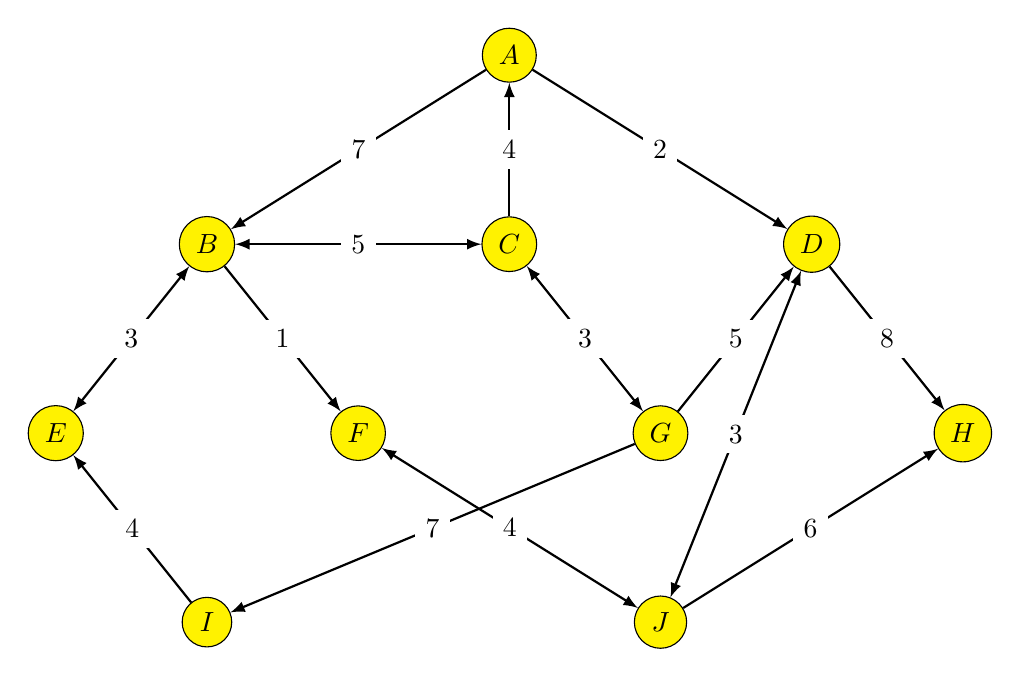
\begin{tikzpicture}[xscale=.8,yscale=.8]
% Styles (MODIFIABLES)
\tikzstyle{fleche}=[<->,>=latex,thick]
\tikzstyle{sfleche}=[->,>=latex,thick]
\tikzstyle{noeud}=[fill=yellow,circle,draw]
\tikzstyle{feuille}=[fill=orange,circle,draw]
\tikzstyle{etiquette}=[midway,fill=white,draw=white]
\tikzstyle{etiquette2}=[rectangle,fill=white,draw=white]
% Dimensions (MODIFIABLES)
\def\DistanceInterNiveaux{3}
\def\DistanceInterFeuilles{2}
% Dimensions calculées (NON MODIFIABLES)
\def\NiveauA{(-0)*\DistanceInterNiveaux}
\def\NiveauB{(-1)*\DistanceInterNiveaux}
\def\NiveauC{(-2)*\DistanceInterNiveaux}
\def\NiveauD{(-3)*\DistanceInterNiveaux}
\def\InterFeuilles{(1.2)*\DistanceInterFeuilles}
% Noeuds (MODIFIABLES : Styles et Coefficients d'InterFeuilles)
\node[noeud] (a) at ({(0)*\InterFeuilles},{\NiveauA}) {$A$};
\node[noeud] (b) at ({(-2)*\InterFeuilles},{\NiveauB}) {$B$};
\node[noeud] (c) at ({(0)*\InterFeuilles},{\NiveauB}) {$C$};
\node[noeud] (d) at ({(2)*\InterFeuilles},{\NiveauB}) {$D$};
\node[noeud] (e) at ({(-3)*\InterFeuilles},{\NiveauC}) {$E$};
\node[noeud] (f) at ({(-1)*\InterFeuilles},{\NiveauC}) {$F$};
\node[noeud] (g) at ({(1)*\InterFeuilles},{\NiveauC}) {$G$};
\node[noeud] (h) at ({(3)*\InterFeuilles},{\NiveauC}) {$H$};
\node[noeud] (i) at ({(-2)*\InterFeuilles},{\NiveauD}) {$I$};
\node[noeud] (j) at ({(1)*\InterFeuilles},{\NiveauD}) {$J$};
% Arcs (MODIFIABLES : Styles)
\draw[sfleche] (a)--(b) node[etiquette] {$7$};
\draw[sfleche] (c)--(a) node[etiquette] {$4$};
\draw[sfleche] (a)--(d) node[etiquette] {$2$};
\draw[fleche] (b)--(c) node[etiquette] {$5$};
\draw[fleche] (b)--(e) node[etiquette] {$3$};
\draw[sfleche] (b)--(f) node[etiquette] {$1$};
\draw[fleche] (c)--(g) node[etiquette] {$3$};
\draw[sfleche] (g)--(d) node[etiquette] {$5$};
\draw[sfleche] (d)--(h) node[etiquette] {$8$};
\draw[fleche] (d)--(j) node[etiquette] {$3$};
\draw[sfleche] (i)--(e) node[etiquette] {$4$};
\draw[sfleche] (g)--(i) node[etiquette] {$7$};
\draw[fleche] (f)--(j) node[etiquette] {$4$};
\draw[sfleche] (j)--(h) node[etiquette] {$6$};
\end{tikzpicture}
\end{center}
\item Implémenter en langage Python la fonction \code{parcours\_prof}.
\item L'arbre couvrant d'un graphe est un arbre qui a les mêmes sommets que le graphe et est obtenu en supprimant des arcs afin qu'il n'y ait aucun cycle et qu'il n'existe à chaque fois qu'un unique trajet entre deux sommets. 
\begin{enumerate}
\item Donner un arbre couvrant du graphe ci-dessus.
\item Expliquer comment on peut à partir du parcours en profondeur d'un graphe obtenir un arbre couvrant. 
\end{enumerate}
\end{enumerate}



\newpage
\section*{Exercice 3}
\emph{Cet exercice porte sur la programmation et utilise essentiellement de la Programmation Orientée Objet et les tableaux en langage Python.}\\
Un capteur est placé sur un moteur et commence à prendre des mesures de température à la mise en route de celui-ci.\\
Une mesure est stockée sous la forme d'un objet défini au moyen du constructeur suivant 
\begin{Python}
class mesure :
    def __init__(t,x):
        '''t : temps en secondes depuis la mise en route 
          x est la température mesurée (en deg. celsius)'''
        self.duree=t
        self.temp=x
\end{Python} 
\subsection*{\vskip - 7 mm Question 1}
\begin{enumerate}
\item Comment s'appellent \code{duree} et \code{temps} ?
\item Quelle instruction permet de créer une mesure \code{m} opérée 300 secondes après la mise en marche du moteur et indiquant une température de 275 degrés ? 
\item On a exécuté l'instructions \code{m1=mesure(730,200)}.\\
Que renvoie l'instruction \code{m1.duree} ? Que renvoie l'instruction \code{m1.temp>250} ? 
\item Pour plus de lisibilité, on veut pouvoir accéder au temps écoulé sous la forme d'un 3-uplet donnant les heures, les minutes et les secondes. 
\begin{enumerate}
\item A la main, convertir une durée de 7545 secondes en heures/minutes/secondes.
\item Compléter le code de la fonction suivante prévue à cet effet. \\
On rappelle que \code{//} donne le quotient de la division de deux entiers et \code{\%} donne le reste de la division de deux entiers. Ainsi, \code{10000//3600=2} et \code{10000\%3600=2800}
\begin{Python}
	def chrono(self):
		heures= #à compléter1
		secondes_restantes=#à compléter2
		minutes=#à compléter3
		secondes=#à compléter4
		return(heures,minutes,secondes)       
\end{Python} 
\item Comment s'appelle une fonction qui comme \code{chrono}, s'applique spécifiquement aux éléments d'une classe ?
\end{enumerate}
\end{enumerate}
On dispose maintenant de toute une série de mesures, mises dans un tableau Python \code{t}. 
\subsection*{\vskip - 7 mm Question 2}
On a exécuté les commandes suivantes : 
\begin{Python}
t=[]
t.append(mesure(0,17))
t.append(mesure(10,100))
t.append(mesure(20,210))
t.append(mesure(30,215))
t.append(mesure(40,217))
t.append(mesure(50,213))
\end{Python}
\begin{enumerate}
\item Que renvoient les appels 
\code{t[1]}  \hskip 1cm \code{t[2].duree} \hskip 1cm \code{t[4].temp} \hskip 1cm \code{t[6].temp}  ?
\item Au vu de ces données, décrire brièvement le protocole de mesure et les résultats observés
\item Compléter le code de la fonction \code{depassement} prenant comme paramètre \code{t} un tableau de mesures et une valeur \code{a} et renvoyant un tableau contenant les horaires (en seconde) auxquels la température mesurée a dépassé \code{a}.
\begin{Python}
# à compléter1
	val_dep=[]
	for mesu in t :
		if # à compléter2 
			val_dep.# à compléter3
	return(val_dep)
\end{Python}
\item Ecrire le code d'une fonction \code{temperature\_moy} prenant comme paramètre un tableau \code{t} de mesures et renvoyant la température moyenne relevée. 
\end{enumerate}
On s'intéresse maintenant aux problèmes de surchauffe du moteur et aux laps de temps pendant lesquels la température moteur dépasse une certaine valeur. On considère ainsi le code suivant : 
\begin{Python}
def depassement2(t,a):
	n=len(t)
	for k in range(0,n):
		if t[k].temp>a and t[k+1].temp>a and t[k+2].temp>a :
			return([t[k].duree,t[k+1].duree,t[k+2].duree)
	return('ok')
\end{Python}
En l'état, lorsqu'on l'exécute avec \code{t} un tableau de mesures et \code{a} un nombre, il donne parfois un message d'erreur du type \code{IndexError: list index out of range}
\subsection*{\vskip - 9 mm Question 3}
\begin{enumerate}
\item \begin{enumerate}
\item Justifier cette situation (existence et caractère non systématique de l'erreur).
\item Proposer une modification du programme permettant d'éviter cela.
\item Le programme ayant été corrigé, décrire simplement ce qu'il fait. En particulier, quand renvoie-t-il \code{'ok'} ?   
\end{enumerate}
\item \begin{enumerate}
\item Avec \code{len(t)=n}, combien de tests effectue au maximum la fonction \code{depassement2} ? 
\item Est-ce que tous ces tests sont utiles ? Pourquoi ?
\item On propose alors l'algorithme suivant, écrit en pseudo-code :
{\small \begin{Python}
Fonction depassement3(t,a)
n=longueur de t
c=0
k=0
Tant que c<3 et k<n
Si la température de la mesure t[k] est >a
Alors c=c+1
Sinon c=0
Fin Si
k=k+1
Fin Tant que       
Si c vaut 3 
Alors  # à compléter1
Sinon # à compléter2
Fin Si
\end{Python}}
Traduire en langage Python cet algorithme en complétant les deux lignes afin que \code{depassement2} et \code{depassement3} fournissent le même résultat.
\end{enumerate}
\end{enumerate}
%
%
%
%
\newpage
\section*{Exercice 4}
\emph{Cet exercice porte sur les bases de données relationnelles et sur le langage SQL.}


Vous êtes un nouvel ingénieur, embauché par la Compagnie des Trains Rapides (CTR) et votre mission consiste à définir les caractéristiques du réseau ferroviaire régional de cette compagnie, ainsi que des trains qui y circulent. Cela sera utilisé par exemple pour afficher sur les écrans d'information d'une gare les horaire des trains qui vont la desservir.


\begin{figure}[ht]
\centering
\includegraphics[width=12cm]{images/reseauFerre.JPG}
\caption{Schéma du réseau ferroviaire régional}
\end{figure}

%%%%%%%%%%%%%%%%%%%%%%%%%%%%%%%%%%%%%%%%%%%%%%%%%%%%%%%%%%%%%%%%%%%%%%%%%%
\subsection*{Question 1}
%%%%%%%%%%%%%%%%%%%%%%%%%%%%%%%%%%%%%%%%%%%%%%%%%%%%%%%%%%%%%%%%%%%%%%%%%%

Dans une première approche de votre mission, vous décidez de concevoir un tableau qui indique les gares desservies par chaque train. Le tableau a la forme suivante : 



\begin{center}
\begin{tabular}[c]{c|c|c|c|c}
IdTrain & NumLigne & Sens & NomGare & Horaire \\ \hline
AZ341 & 1 & + & B & 08:50 \\ \hline
AZ341 & 1 & + & C & 09:20 \\ \hline
DE666 & 2 & - & J & 13:20 \\ \hline
DE666 & 2 & - & D & 14:40 \\ \hline
... & ... & ... & ... & ... \\ \hline
\end{tabular}
\end{center}

\begin{enumerate}
 \item Citez trois problèmes qui peuvent se poser avec un tel tableau, lors de la création, l'utilisation ou la modification des données de ce tableau.
 \item Vous décidez rapidement qu'une bien meilleure approche consiste à stocker ces données à l'aide d'une base de données relationnelle. Citez trois exemples concrets (hors traffic ferroviaire) où des bases de données sont utilisées.
\end{enumerate}




%%%%%%%%%%%%%%%%%%%%%%%%%%%%%%%%%%%%%%%%%%%%%%%%%%%%%%%%%%%%%%%%%%%%%%%%%%
\subsection*{Question 2}
%%%%%%%%%%%%%%%%%%%%%%%%%%%%%%%%%%%%%%%%%%%%%%%%%%%%%%%%%%%%%%%%%%%%%%%%%%

La base de données que vous avez conçu est décrit par le schéma relationnel suivant :
\begin{itemize}
 \item \textsc{Gare} (\underline{Nom} (string), CorrespBus\footnote{Indique s'il y a une correspondance possible avec des bus.} (boolean))
 \item \textsc{Ligne} (\underline{Num} (integer), \emph{NomGareDebut} (string))
 \item \textsc{Train} (\underline{Id} (string), \emph{NumLigne} (integer), Sens (string))
 \item \textsc{Reseau} (\underline{\emph{NomGare}} (string), \underline{\emph{NumLigne}} (integer), PtKilometriq\footnote{Indique la distance de la gare à la gare de début de ligne, en km, dans le sens '+'.} (integer))
 \item \textsc{Desserte} (\underline{Id} (integer), \emph{NomGare} (string), \emph{IdTrain} (string), Horaire\footnote{Le format de l'horaire est HH:MM} (time))
\end{itemize}

\begin{enumerate}
 \item Quel nom donne-t-on aux différents termes tels que \verb'Id', \verb'CorrespBus', ou \verb'Horaire' ? Quel nom donne-t-on à une ligne présente dans une relation ?
 \item D'après vous, que représentent les termes soulignés ? Quel rôle joue ce type de terme dans une relation ?
 \item D'après vous, que représentent les termes en italique ?
\end{enumerate}


%%%%%%%%%%%%%%%%%%%%%%%%%%%%%%%%%%%%%%%%%%%%%%%%%%%%%%%%%%%%%%%%%%%%%%%%%%
\subsection*{Question 3}
%%%%%%%%%%%%%%%%%%%%%%%%%%%%%%%%%%%%%%%%%%%%%%%%%%%%%%%%%%%%%%%%%%%%%%%%%%

La base de données est supposée déjà partiellement remplie. Mais il faut régulièrement la mettre à jour, suite à certains évènements.

\begin{enumerate}
 \item Un nouveau train va être mis en circulation sur la ligne 1, dans le sens '-'. Son identifiant est 'PP1234'. Ce train part à 08:00 de la gare 'I' et arrive à 10:00 à la gare 'G', en desservant à 09:00 la gare 'D'. Ecrire, à l'aide de la commande \verb'INSERT INTO', les commandes SQL ajoutant toutes ces informations dans la BDD. On rappelle que la syntaxe d'utilisation de cette commande est : 
 \begin{verbatim}
  INSERT INTO nom_de_la_table VALUES (valeur_1, valeur_2, ...)
 \end{verbatim}
 A noter que l'identifiant de desserte est automatiquement incrémenté lors de l'ajout d'une nouvelle desserte et n'a donc pas besoin d'être précisé.
 \item Le train 'FX0102', desservant toutes les gares de la ligne 3 dans le sens '+', ne peut démarrer à cause d'un problème technique. Vous décidez de le supprimer à l'aide de la commande SQL suivante : 
 \begin{verbatim}
  DELETE FROM Train WHERE Id = 'FX0102'
 \end{verbatim}
 Mais le Système de Gestion de Bases de Données (SGBD) refuse d'exécuter cette commande et renvoie un message d'erreur (alors que la syntaxe est bien correcte). Expliquez pourquoi ? Proposez une solution à ce problème.
 \item Vous apprenez que le train 'ZE6321' de la ligne 2 en sens '+' doit ralentir après la gare 'J' et arrivera à 13:10 à la gare 'E', au lieu de 12:50. Ecrire, à l'aide de la commande \verb'UPDATE', la ou les commandes SQL mettant à jour ces informations dans la BDD. On rappelle que la syntaxe d'utilisation de cette commande est : 
 \begin{verbatim}
  UPDATE nom_de_la_table 
  SET nom_de_col1 = valeur1, nom_de_col2 = valeur2, ... 
  WHERE condition
 \end{verbatim}
\end{enumerate}



%%%%%%%%%%%%%%%%%%%%%%%%%%%%%%%%%%%%%%%%%%%%%%%%%%%%%%%%%%%%%%%%%%%%%%%%%%
\subsection*{Question 4}
%%%%%%%%%%%%%%%%%%%%%%%%%%%%%%%%%%%%%%%%%%%%%%%%%%%%%%%%%%%%%%%%%%%%%%%%%%

Dans cette question, vous devez écrire des requêtes SQL permettant de renvoyer des informations exigées, à l'aide des seules commandes SQL suivantes : \verb'WHERE', \verb'MAX', \verb'DISTINCT', \verb'COUNT', \verb'AS', \verb'FROM', \verb'SELECT', \verb'JOIN', \verb'ON', \verb'ORDER BY', \verb'LIMIT', \verb'SUM', \verb'DESC', \verb'OFFSET', \verb'MIN'. Vous pouvez également effectuer des sous-requêtes ou des requêtes imbriquées, si besoin est.

\begin{enumerate}
 \item Afficher toute la table \textsc{Train}.
 \item Afficher les noms de toutes les gares du réseau régional, avec un tri selon l'ordre alphabétique croissant.
 \item Afficher le nombre de toutes les gares qui possèdent une correspondance avec un réseau de bus.
 \item Afficher le nom et la position kilométrique de toutes les gares de la ligne 3, avec un tri selon l'ordre croissant des positions kilométriques.
 \item Afficher, sans répétition, le numéro des lignes qui passent par la gare 'J'.
 \item Afficher la longueur totale de la ligne 1.
 \item Afficher le nom de tous les trains qui desservent la gare 'D' selon le sens '+'. Attention, on ne veut pas de répétition de noms de train (ce qui peut avoir lieu si un train passe plusieurs fois par cette gare dans ce sens, au cours de la journée).
 \item Afficher, sans répétition de train, le nombre de trains qui circulent sur la ligne 3, après 20:00.
\end{enumerate}
%
%
%
%
\newpage
\section*{Exercice 5}
\emph{Cet exercice comporte trois parties indépendantes portant sur les commandes Linux et les protocoles réseaux.}
\subsection*{Partie 1 : Commandes Linux}
On rappelle les commandes suivantes : \medskip\\
\begin{tabular}{|l|l|}\hline
Commande & Description \\ \hline
\code{pwd} & Affiche le nom du répertoire courant \\ \hline
\code{ls} & Liste le contenu du répertoire courant \\ \hline
\code{cd}  & Change de répertoire courant  \\ \hline
\code{mkdir}& Crée un nouveau répertoire  \\ \hline
\code{cp}& Crée une copie d'un fichier ou d'un répertoire \\ \hline
\code{rm}& Supprime un répertoire ou un fichier \\ \hline
\code{touch}& Crée un fichier (entre autres choses) \\ \hline\hline
\code{*.*}& Désigne le contenu complet d'un répertoire. \\ \hline
\end{tabular}\medskip\\
A noter que ces commandes s'utilisent avec des attributs, en particuliers des noms de répertoires/fichiers et des chemins d'accès. On distingue ainsi : 
\begin{itemize}
\item les chemins absolus, donnés à partir de la racine, commençant par $/$
\item les chemins relatifs, donnés à partir de la position actuelle, commençant par le nom du premier répertoire.
\end{itemize}
Ainsi, si on dispose d'un système de fichier avec l'arborescence suivante, 
\begin{figure}[ht]
\centering
\includegraphics[width=14cm]{images/arbre2.JPG}
\caption{Arborescence \label{arbo}}
\end{figure}
\begin{itemize}
\item En partant de la racine \code{C}, \code{cd /rep1/rep4/rep7} et \code{cd rep1/rep4/rep7}  mènent dans \code{rep7}. Comme on démarre de la racine, il n'y a pas de différence entre chemin relatif et absolu.
\item Une fois dans \code{rep7}, \code{cd ../../rep6} mène dans \code{rep6} (le \code{..} signifie reculer d'un rang dans l'arborescence).
\item Une fois dans \code{rep6}, la commande \code{cd /rep2} mène directement dans \code{rep2}. Commençant par un \code{/}, c'est un chemin absolu démarrant à la racine.  
\item De même, \code{mkdir /rep2/rep8} créera un répertoire \code{rep8} à l'intérieur de \code{rep2}, peu importe l'endroit depuis lequel la commande est lancée.
\item Tandis que si on est dans \code{rep7}, 
\begin{itemize}
\item \code{touch ../../essai.txt} créera un fichier \code{essai.txt} à l'intérieur de \code{rep1}
\item \code{mkdir rep9} créera un répertoire \code{rep9} dans \code{rep7}
\item \code{mkdir /rep10} créera un répertoire \code{rep10} directement à la racine
\end{itemize}
\end{itemize}
%%%%%%%%%%%%%%%%%%%%%%%%%%%%%%%%%%%%%%%%%%%%%%%%%%%%%%%%%%%%%%%%%%%%%%%%%%
\subsection*{Question 1}
%%%%%%%%%%%%%%%%%%%%%%%%%%%%%%%%%%%%%%%%%%%%%%%%%%%%%%%%%%%%%%%%%%%%%%%%%%
\begin{enumerate}
\item On suppose que :
\begin{itemize}
\item Tous les dossiers et fichiers de la Figure \ref{arbo} ont été crées, sauf la partie encadrée.
\item On vient de taper la commande \code{pwd} dans le shell et on a obtenu comme réponse \code{/rep3}.
\end{itemize}
\vskip 3mm
Donner un jeu de commandes permettant de créer les dossiers et les fichiers de la partie encadrée.
\item On suppose maintenant que tous les dossiers et fichiers de la Figure \ref{arbo} ont été créées.\\
On entre alors les commandes suivantes en console : 
\begin{Python}
rm /rep2
cd /rep1/rep4/rep7
cp *.* /rep3
cp ../../rep6/*.*  /rep3
cd ..
cd ..
rm *.*
\end{Python}
Dessiner, en justifiant brièvement, l'arborescence résultant de ces opérations. 
\end{enumerate}
\subsection*{Partie 2 : Protocole RIP}
On considère le réseau suivant (chaque routeur est repéré par une lettre) :
\begin{center}
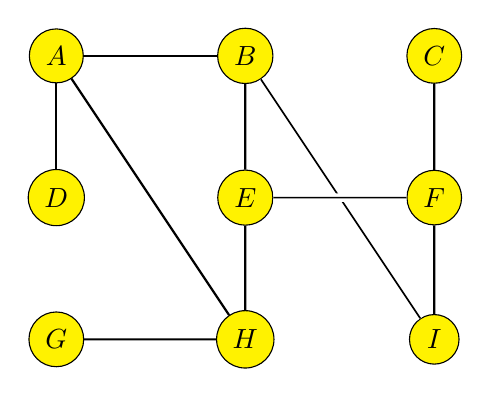
\begin{tikzpicture}[xscale=0.8,yscale=0.8]
% Styles (MODIFIABLES)
\tikzstyle{fleche}=[-,>=latex,thick]
\tikzstyle{noeud}=[fill=yellow,circle,draw]
\tikzstyle{feuille}=[fill=orange,circle,draw]
% Dimensions (MODIFIABLES)
\def\DistanceInterNiveaux{3}
\def\DistanceInterFeuilles{2}
% Dimensions calculées (NON MODIFIABLES)
\def\NiveauA{(-0)*\DistanceInterNiveaux}
\def\NiveauB{(-.75)*\DistanceInterNiveaux}
\def\NiveauC{(-1.5)*\DistanceInterNiveaux}
\def\InterFeuilles{(.75)*\DistanceInterFeuilles}
% Noeuds (MODIFIABLES : Styles et Coefficients d'InterFeuilles)
\node[noeud] (Ra) at ({(0)*\InterFeuilles},{\NiveauA}) {$A$};
\node[noeud] (Rb) at ({(2)*\InterFeuilles},{\NiveauA}) {$B$};
\node[noeud] (Rc) at ({(4)*\InterFeuilles},{\NiveauA}) {$C$};
\node[noeud] (Rd) at ({(0)*\InterFeuilles},{\NiveauB}) {$D$};
\node[noeud] (Re) at ({(2)*\InterFeuilles},{\NiveauB}) {$E$};
\node[noeud] (Rf) at ({(4)*\InterFeuilles},{\NiveauB}) {$F$};
\node[noeud] (Rg) at ({(0)*\InterFeuilles},{\NiveauC}) {$G$};
\node[noeud] (Rh) at ({(2)*\InterFeuilles},{\NiveauC}) {$H$};
\node[noeud] (Ri) at ({(4)*\InterFeuilles},{\NiveauC}) {$I$};
% Arcs (MODIFIABLES : Styles)
\draw[fleche] (Ra)--(Rb);
\draw[fleche] (Ra)--(Rd);
\draw[fleche] (Ra)--(Rh);
\draw[fleche] (Rb)--(Re);
\draw[fleche,draw=white,double=black,very thick] (Rb)--(Ri);
\draw[fleche] (Rc)--(Rf);
\draw[fleche,draw=white,double=black,very thick] (Re)--(Rf);
\draw[fleche] (Re)--(Rh);
\draw[fleche] (Rf)--(Ri);
\draw[fleche] (Rg)--(Rh);
\end{tikzpicture}
\end{center}
Pour les questions suivantes, on se place dans le cadre du protocole RIP.\\
Pour départager des chemins de même longueur, on considère qu'à chaque fois que cela était possible, les connexions ont été établies dans l'ordre alphabétique. \\
Ainsi, la liaison entre \code{A} et \code{B} a été créée avant celle entre \code{A} et \code{D},...\\
De plus, un chemin entre deux routeurs est remplacé par un autre chemin uniquement si le nouveau chemin est strictement plus court.
\subsection*{Question 2}
\begin{enumerate}
    \item Quel est le chemin de A vers F ?
    \item Recopier sur votre copie et compléter la table de routage du routeur B (sur le modèle de la table du {\bf 3)}:
    \begin{center}
        \begin{tabular}{|c|c|c|}\hline
            Destination&Routeur suivant&Distance\\ \hline
            $\vdots$ &$\vdots$&$\vdots$\\ \hline
            
        \end{tabular}
    \end{center}
    \item Une liaison directe a été ajoutée entre deux routeurs.
    La nouvelle table de routage du routeur F est alors :
    \begin{center}
        \begin{tabular}{|c|c|c|}\hline
            Destination&Routeur suivant&Distance\\ \hline
            A&E &3 \\ \hline
            B&E &2 \\ \hline
            C&C &1 \\ \hline
            D&I &2 \\ \hline
            E&E &1 \\ \hline
            G&E &3 \\ \hline
            H&E &2 \\ \hline
            I&I &1 \\ \hline
        \end{tabular}
    \end{center}
    Entre quels routeurs la liaison a-t-elle été ajoutée ? Justifier brièvement.
    
\end{enumerate}
\subsection*{Partie 3 : Protocole OSPF}
On considère le réseau suivant (chaque routeur est repéré par une lettre) :
\begin{multicols}{2}
\begin{center}
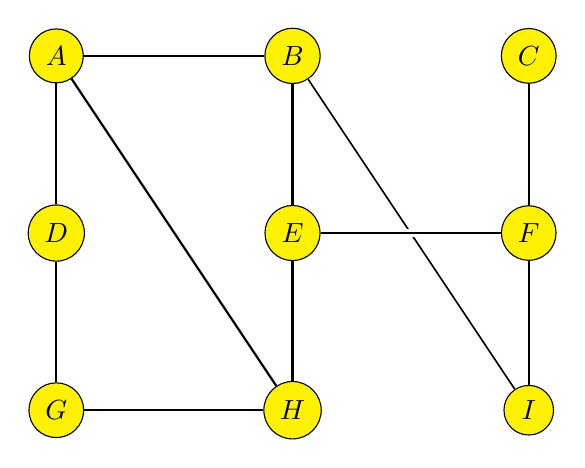
\begin{tikzpicture}[xscale=1,yscale=1]
% Styles (MODIFIABLES)
\tikzstyle{fleche}=[-,>=latex,thick]
\tikzstyle{noeud}=[fill=yellow,circle,draw]
\tikzstyle{feuille}=[fill=orange,circle,draw]
% Dimensions (MODIFIABLES)
\def\DistanceInterNiveaux{3}
\def\DistanceInterFeuilles{2}
% Dimensions calculées (NON MODIFIABLES)
\def\NiveauA{(-0)*\DistanceInterNiveaux}
\def\NiveauB{(-.75)*\DistanceInterNiveaux}
\def\NiveauC{(-1.5)*\DistanceInterNiveaux}
\def\InterFeuilles{(.75)*\DistanceInterFeuilles}
% Noeuds (MODIFIABLES : Styles et Coefficients d'InterFeuilles)
\node[noeud] (Ra) at ({(0)*\InterFeuilles},{\NiveauA}) {$A$};
\node[noeud] (Rb) at ({(2)*\InterFeuilles},{\NiveauA}) {$B$};
\node[noeud] (Rc) at ({(4)*\InterFeuilles},{\NiveauA}) {$C$};
\node[noeud] (Rd) at ({(0)*\InterFeuilles},{\NiveauB}) {$D$};
\node[noeud] (Re) at ({(2)*\InterFeuilles},{\NiveauB}) {$E$};
\node[noeud] (Rf) at ({(4)*\InterFeuilles},{\NiveauB}) {$F$};
\node[noeud] (Rg) at ({(0)*\InterFeuilles},{\NiveauC}) {$G$};
\node[noeud] (Rh) at ({(2)*\InterFeuilles},{\NiveauC}) {$H$};
\node[noeud] (Ri) at ({(4)*\InterFeuilles},{\NiveauC}) {$I$};
% Arcs (MODIFIABLES : Styles)
\draw[fleche] (Ra)--(Rb);
\draw[fleche] (Ra)--(Rd);
\draw[fleche] (Ra)--(Rh);
\draw[fleche] (Rb)--(Re);
\draw[fleche] (Rd)--(Rg);
\draw[fleche,draw=white,double=black,very thick] (Rb)--(Ri);
\draw[fleche] (Rc)--(Rf);
\draw[fleche,draw=white,double=black,very thick] (Re)--(Rf);
\draw[fleche] (Re)--(Rh);
\draw[fleche] (Rf)--(Ri);
\draw[fleche] (Rg)--(Rh);
\end{tikzpicture}
\end{center}

\begin{tabular}{|l|l|l|}\hline
    Liaison& Type   & Débit\\\hline
    A$\leftrightarrow$B&Bluetooth&5 Mbit/s \\\hline
    A$\leftrightarrow$D&Ethernet&20 Mbit/s \\\hline
    A$\leftrightarrow$H&Fibre&1 Gbit/s \\\hline
    B$\leftrightarrow$E&Bluetooth&5 Mbit/s\\\hline
    B$\leftrightarrow$I&Fast Ethernet&100 Mbit/s\\\hline
    C$\leftrightarrow$F&Fibre&1 Gbit/s \\\hline
   D$\leftrightarrow$G&Fast Ethernet&100 Mbit/s  \\\hline
    E$\leftrightarrow$F&Wi-Fi&200 Mbit/s \\\hline
	E$\leftrightarrow$H&Fast Ethernet&100 Mbit/s \\\hline
    F$\leftrightarrow$I&Ethernet&20 Mbit/s \\\hline
    G$\leftrightarrow$H&Ethernet&10 Mbit/s \\\hline
    \end{tabular}
\end{multicols}
Pour les questions suivantes, on se place dans le cadre du protocole OSPF.
On rappelle que pour ce protocole, le coût d'une liaison est 
$\text{coût}=\frac{10^8}{d}$ où $d$ est la bande passante en $bit/s$.
\subsection*{Question 3}
\begin{enumerate}
    \item Quel est le coût des liaisons AB et AH ? Détailler les calculs.
    \item Sans autres justifications, recopier sur votre copie le graphe et donner la pondération de chacun des arcs. 
    \item Quel est le coût total du chemin D-A-B-E ?
    \item En justifiant brièvement, quel est le chemin le moins coûteux allant de G à B ?
\end{enumerate}

\end{document}

